Generally, research in Language \& Vision (L\&V) is interested in modeling how speakers \textit{naturally} name, refer to or talk about visual objects and scenes, in contrast to predicting abstract object labels as e.g.\ in Computer Vision. With the recent explosion of interest in this area, a number of (massive) data collections for various language \& vision (L\&V) tasks have become available: these range from image captioning data \cite{fangetal:2015,devlin:imcaqui,Bernardietal:automatic}, and referring expressions \cite{Kazemzadeh2014,mao15,Yu2016}, to image paragraphs \sz{cite}, multi-modal summaries or visual dialogues \cite{das2017visual,vries2017guesswhat}.
%This typically entails that data collections and models need to account for linguistic variation, as there can hardly ever be a single ground-truth utterance when describing or referring to visual entities. 
%And indeed, variation has been accounted for in the modeling and evaluation of certain L\&V tasks like image captioning \cite{vedantam2015cider,Bernardietal:automatic,dai2017towards}.

In principle, the massive data collections now available in L\&V should not only spur computational, application-oriented research aimed at implementing systems for very specific tasks---they should also constitute extremely valuable resources for research aimed at deriving linguistic generalizations about various phenomena related to language grounding, reference and situated interaction which, for a long time, have been investigated mostly in very controlled and small-domain experimental settings, cf. \cite{anderson1991hcrc,fernangen:sigd07,krahmer:2012,takenobu2012rex,zarriess2016pentoref} for some examples of traditional data collections related to reference and grounding.  
In turn, these linguistic generalizations could inform computational modeling, architecture design and future data collections.
However, so far, studies that have tested linguistic hypotheses on large-scale L\&V resources have been relatively rare. 

In this paper, we take a look at object naming, a basic phenomenon that occurs in virtually every L\&V task and is, at the same time, subject of ongoing research in language grounding and pragmatics. \sz{explain picture naming here?} \sz{briefly say which linguistic questions/hypothesis could be investigated with respect o object naming} But despite the fact that object naming is relatively basic as a phenomenon, we observe that even corpora with massive annotation like VisualGenome~\cite[\vg henceforth]{krishna2016visualgenome} do not provide sufficient information for being able to study object names from a more linguistic perspective ... 

\begin{figure}[tbp]
\scriptsize
\begin{tabular}{p{4.3cm}p{2cm}}
%VisualGenome+ManyNames & \cite{snodgrass}\\
\centering
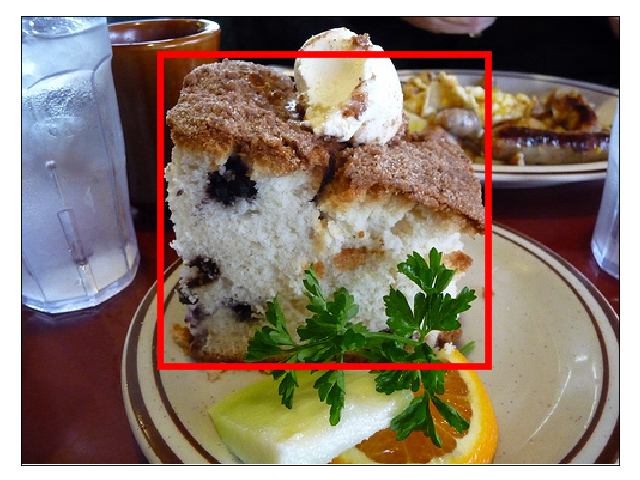
\includegraphics[scale=0.15]{figures/2390077_1254219_supercat_unique.png} &
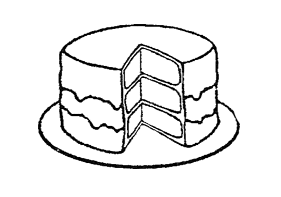
\includegraphics[scale=0.4]{figures/snodgrass_vanderwart_cake_042.png}\\
 cake\ (53),  food\ (19), bread\ (8), burger\ (6), dessert\ (6), snacks\ (3), muffin\ (3),  pastry\ (3) & \hspace{.9cm} cake (83)
\end{tabular}
\caption{Names for a cake object in ManyNames (left) and in cite{snodgrass} (right), percentages of responses in parentheses.}
\label{fig:cake}
\end{figure}


We take a first step at studying natural naming of objects in real-world images and contribute a new dataset, ManyNames, that contains 36 crowd-sourced names for 25K instances from \vg.%
\footnote{The dataset will be available upon publication.}
Thus, our images show objects in complex visual contexts,
unlike the ``clean'' ImageNet data~\cite{imagenet_cvpr09} that has been previously used to train object classifiers \cite{ILSVRC15}, and unlike stylized line drawings used in picture naming experiments in Cognitive Science (see Figure \ref{fig:cake}).

As illustrated for an object of the class ``cake'' in Figure \ref{fig:cake}, our data reveals clear naming preferences (53\% of the annotators prefer the basic-level \textit{cake}) and also rich variation (the remaining annotators prefer other options like \textit{food, dessert, bread}) which is not restricted to taxonomical relations studied in previous work on naming \cite{rosch1976basic,Ordonez:2016,graf2016animal}.

%%% Local Variables:
%%% mode: latex
%%% TeX-master: "lrec2020naming"
%%% End:
